\documentclass[twocolumn]{article}

\usepackage{amsmath}
\usepackage{caption}
\usepackage{graphicx}
\usepackage{float}
\usepackage{subcaption}
\usepackage{gensymb}

% Make table names in captions boldfaced
\captionsetup[table]{labelfont=bf}
\captionsetup[figure]{labelfont=bf}

%opening
\title{Measuring the Zeeman Effect}
\author{}

\begin{document}

\maketitle

\begin{abstract}
	
\end{abstract}

\section{Introduction} \label{sec:Intro}
	\subsection{Historical Background}

	\subsection{Theory of the Zeeman Effect} \label{sec:Theory}
		
\section{Methods and Procedures}
	The Pasco Scientific Model SE-9654 Zeeman Effect Experiment was used to make all observations.
	The experiment consisted of two large solenoids oriented along the same axis with an air gap between them in which a mercury lamp was placed.
	An optical rail was used to align a polarizing filter, a collimating lens, an interference filter, a Fabry-Perot interferometer, and a CMOS camera.
	The basic experimental technique consisted of imaging the interference pattern of the 546.1 nm mercury spectral line through the polarizer and Fabry-Perot interferometer.
	Figure 
	
	\begin{figure*}
		\centering
		\begin{subfigure}{0.5\textwidth}
			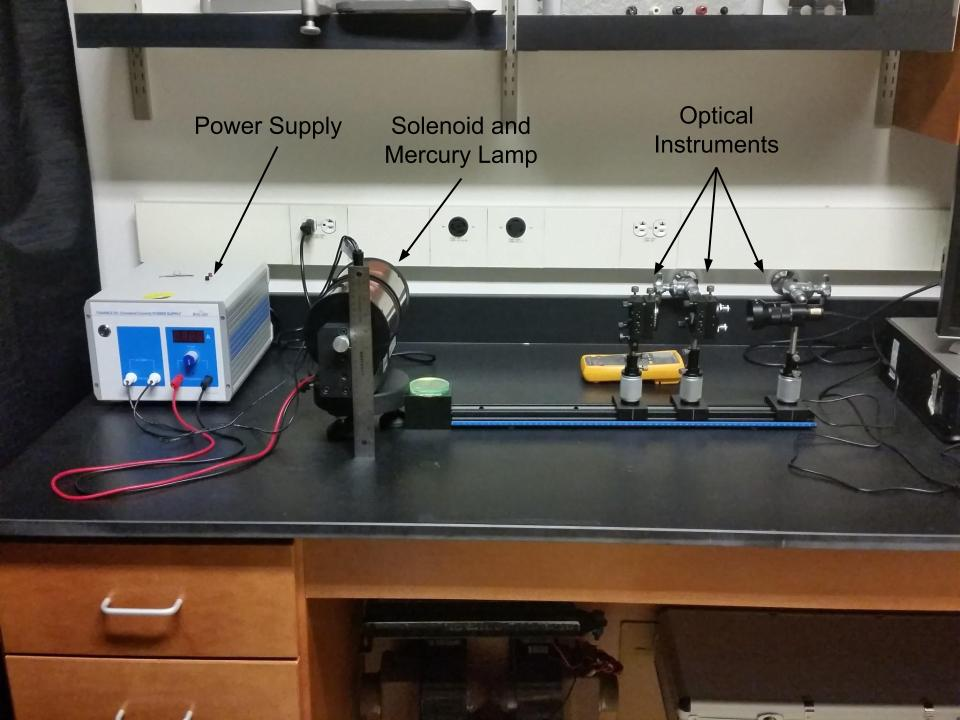
\includegraphics[width = 0.8\textwidth]{Images/ExperimentOverview.jpg}
			\caption{}
			\label{subfig:Overview}
			
		\end{subfigure}%
		\begin{subfigure}{0.5\textwidth}
				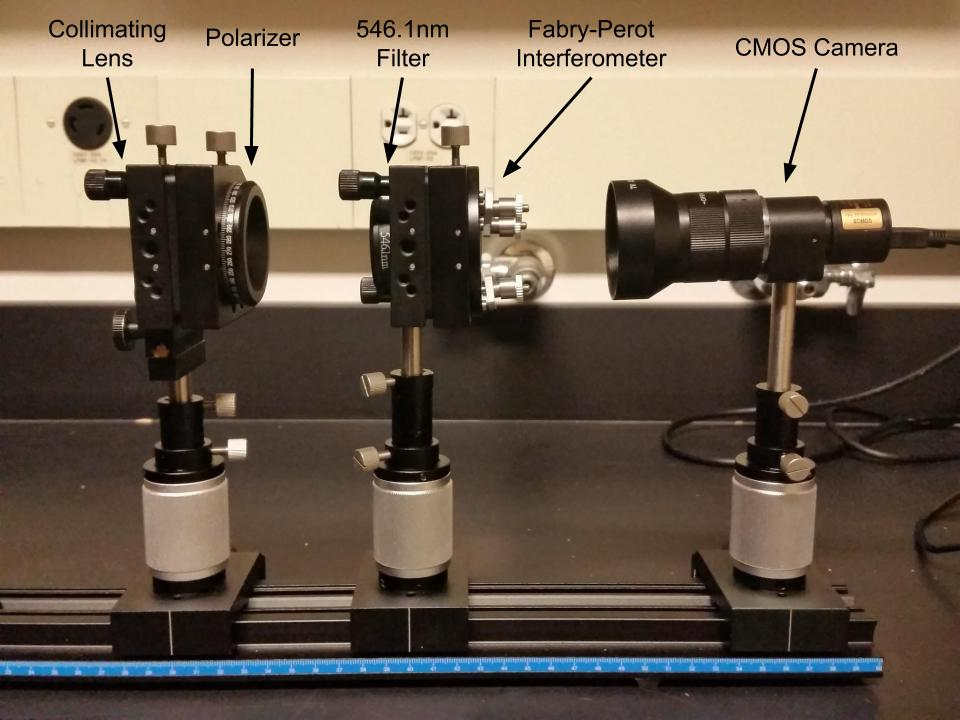
\includegraphics[width = 0.8\textwidth]{Images/OpticsRail.jpg}
				\caption{}
				\label{subfig:OpticsRail}
				
		\end{subfigure}%
		\caption{\textbf{Overview of the Experiment configuration. Figure \ref{subfig:Overview} shows the entire apparatus with the variable power supply for the solenoid and mercury lamp, the solenoid, the mercury lamp (hidden by the solenoid), the optical track, and the optical instruments. Figure \ref{subfig:OpticsRail} shows the optical instruments in detail.}}
		\label{fig:ContextView}
	\end{figure*}
	
	\begin{figure*}
		\centering
		\begin{subfigure}{0.5\textwidth}
			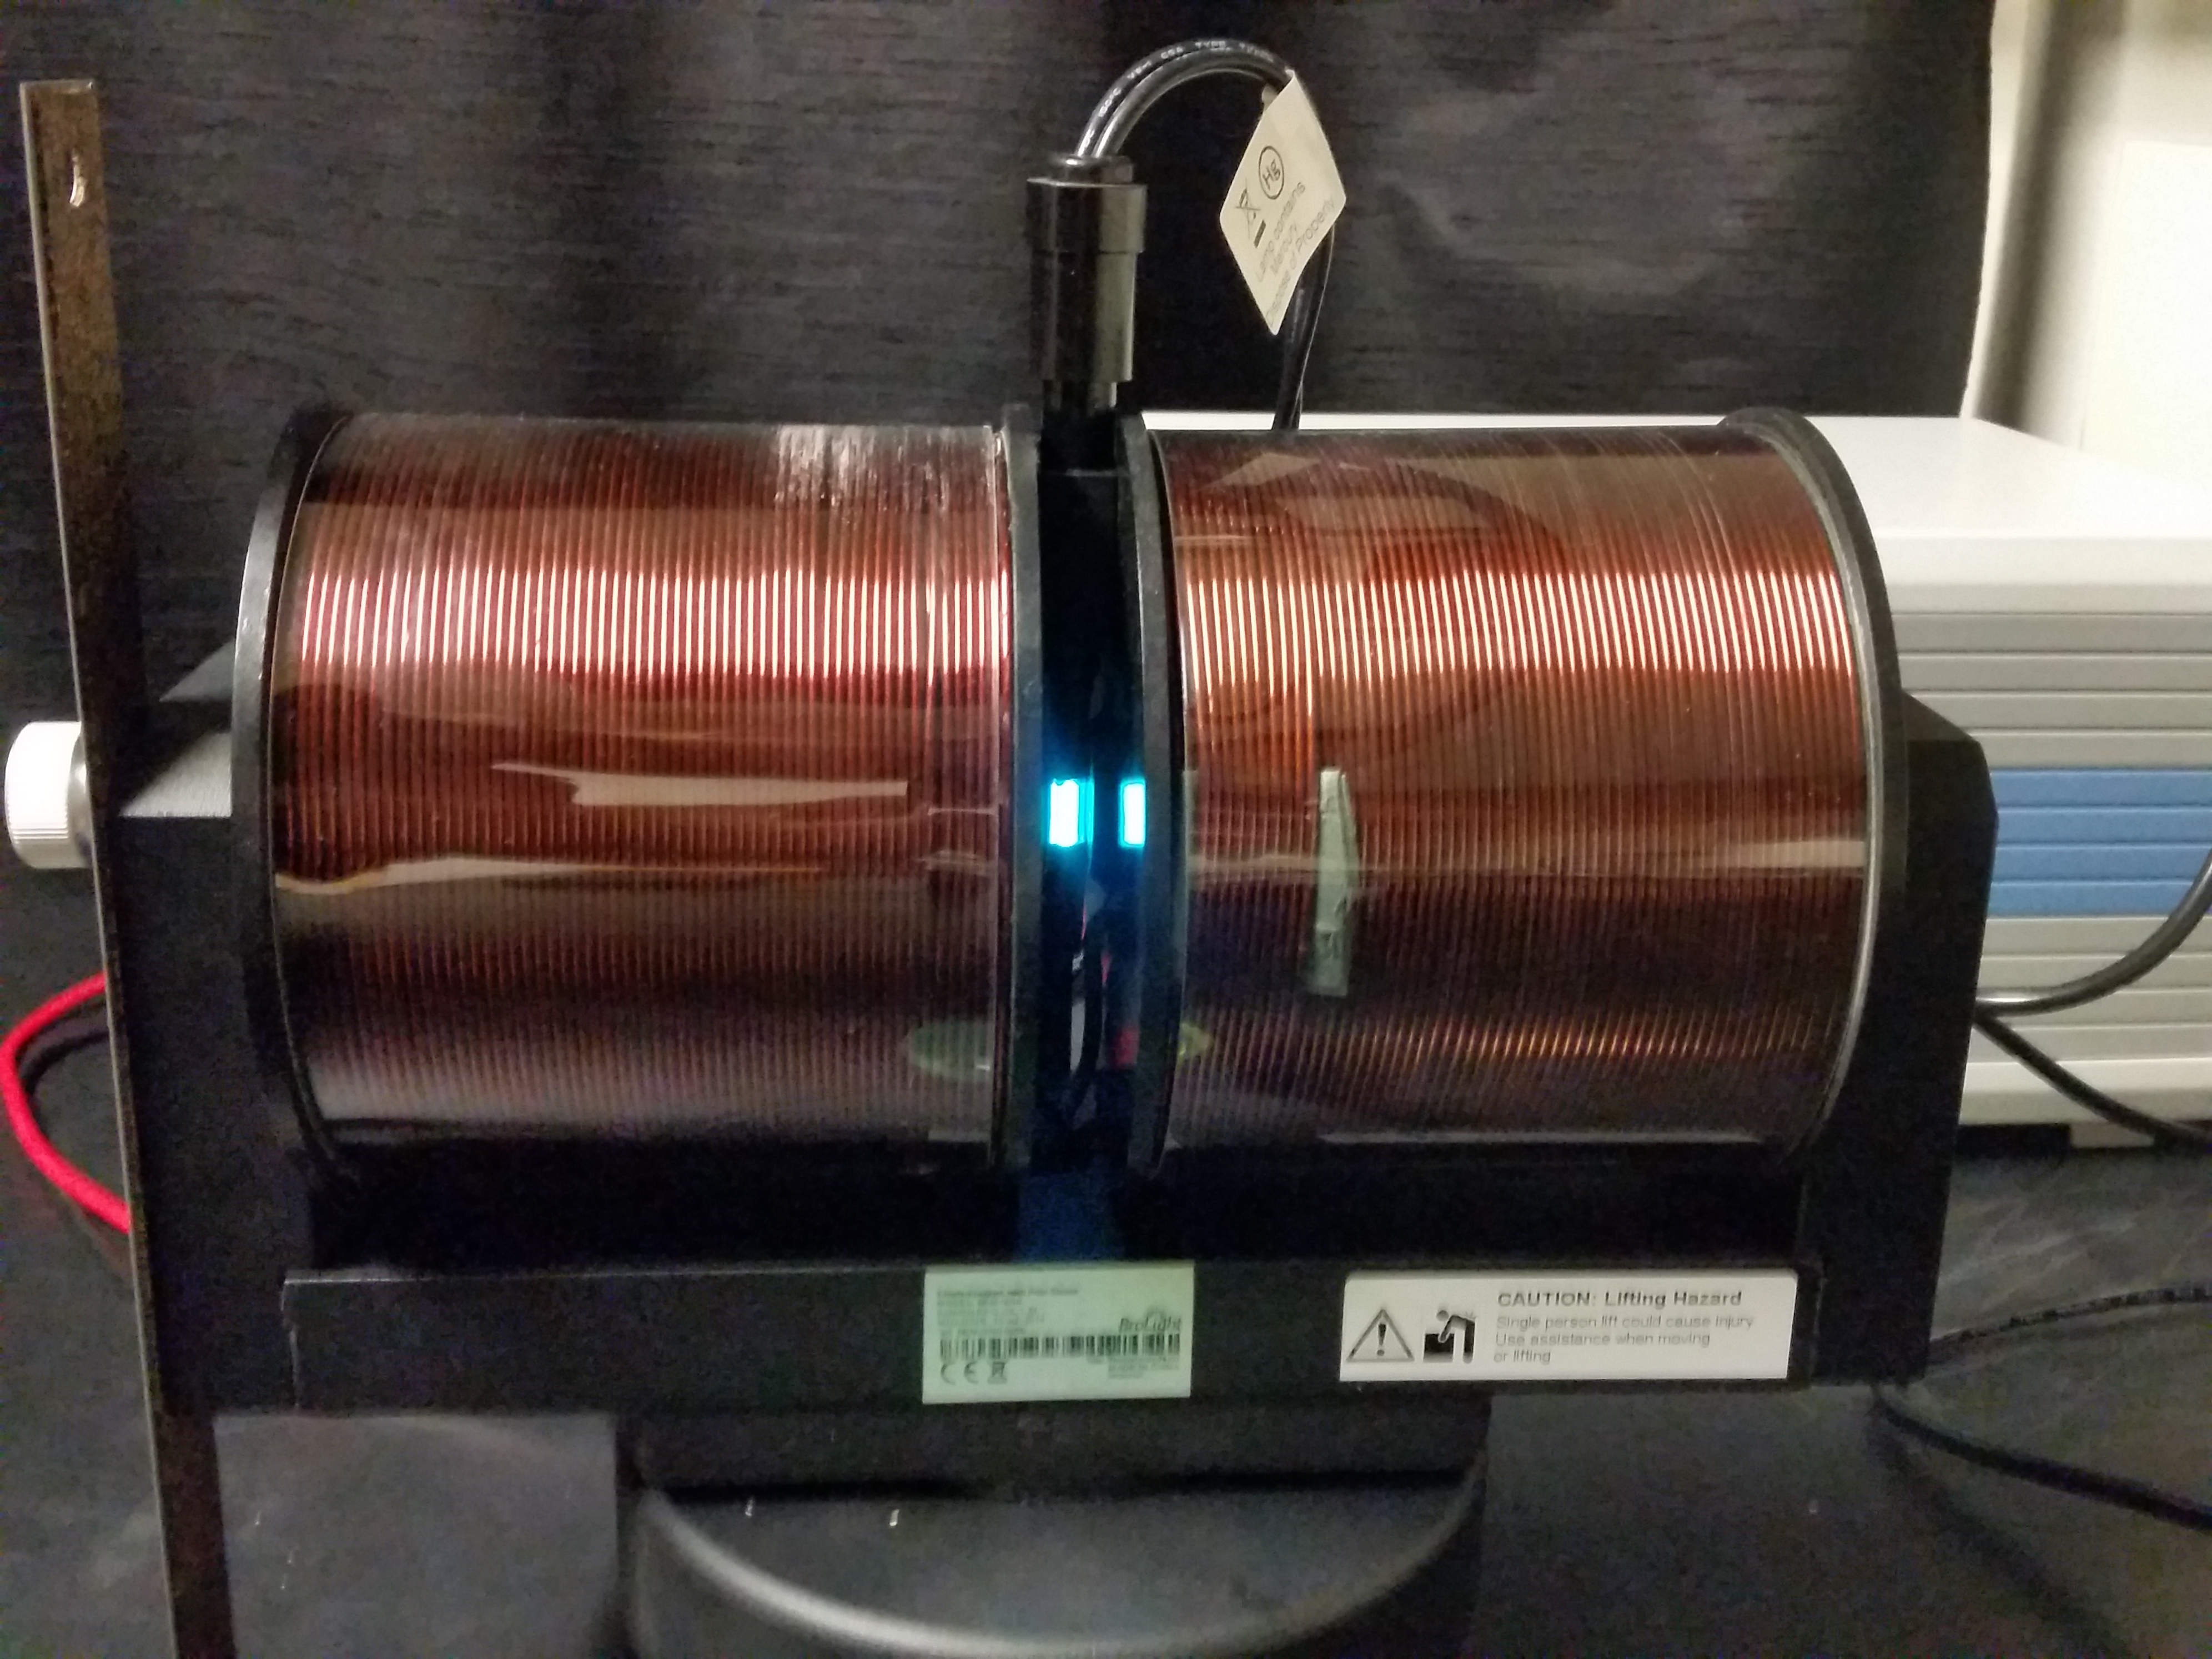
\includegraphics[width = 0.8\textwidth]{Images/PerpendicularView.jpg}
			\caption{}
			\label{subfig:PerpView}
		\end{subfigure}%
		\begin{subfigure}{0.5\textwidth}
			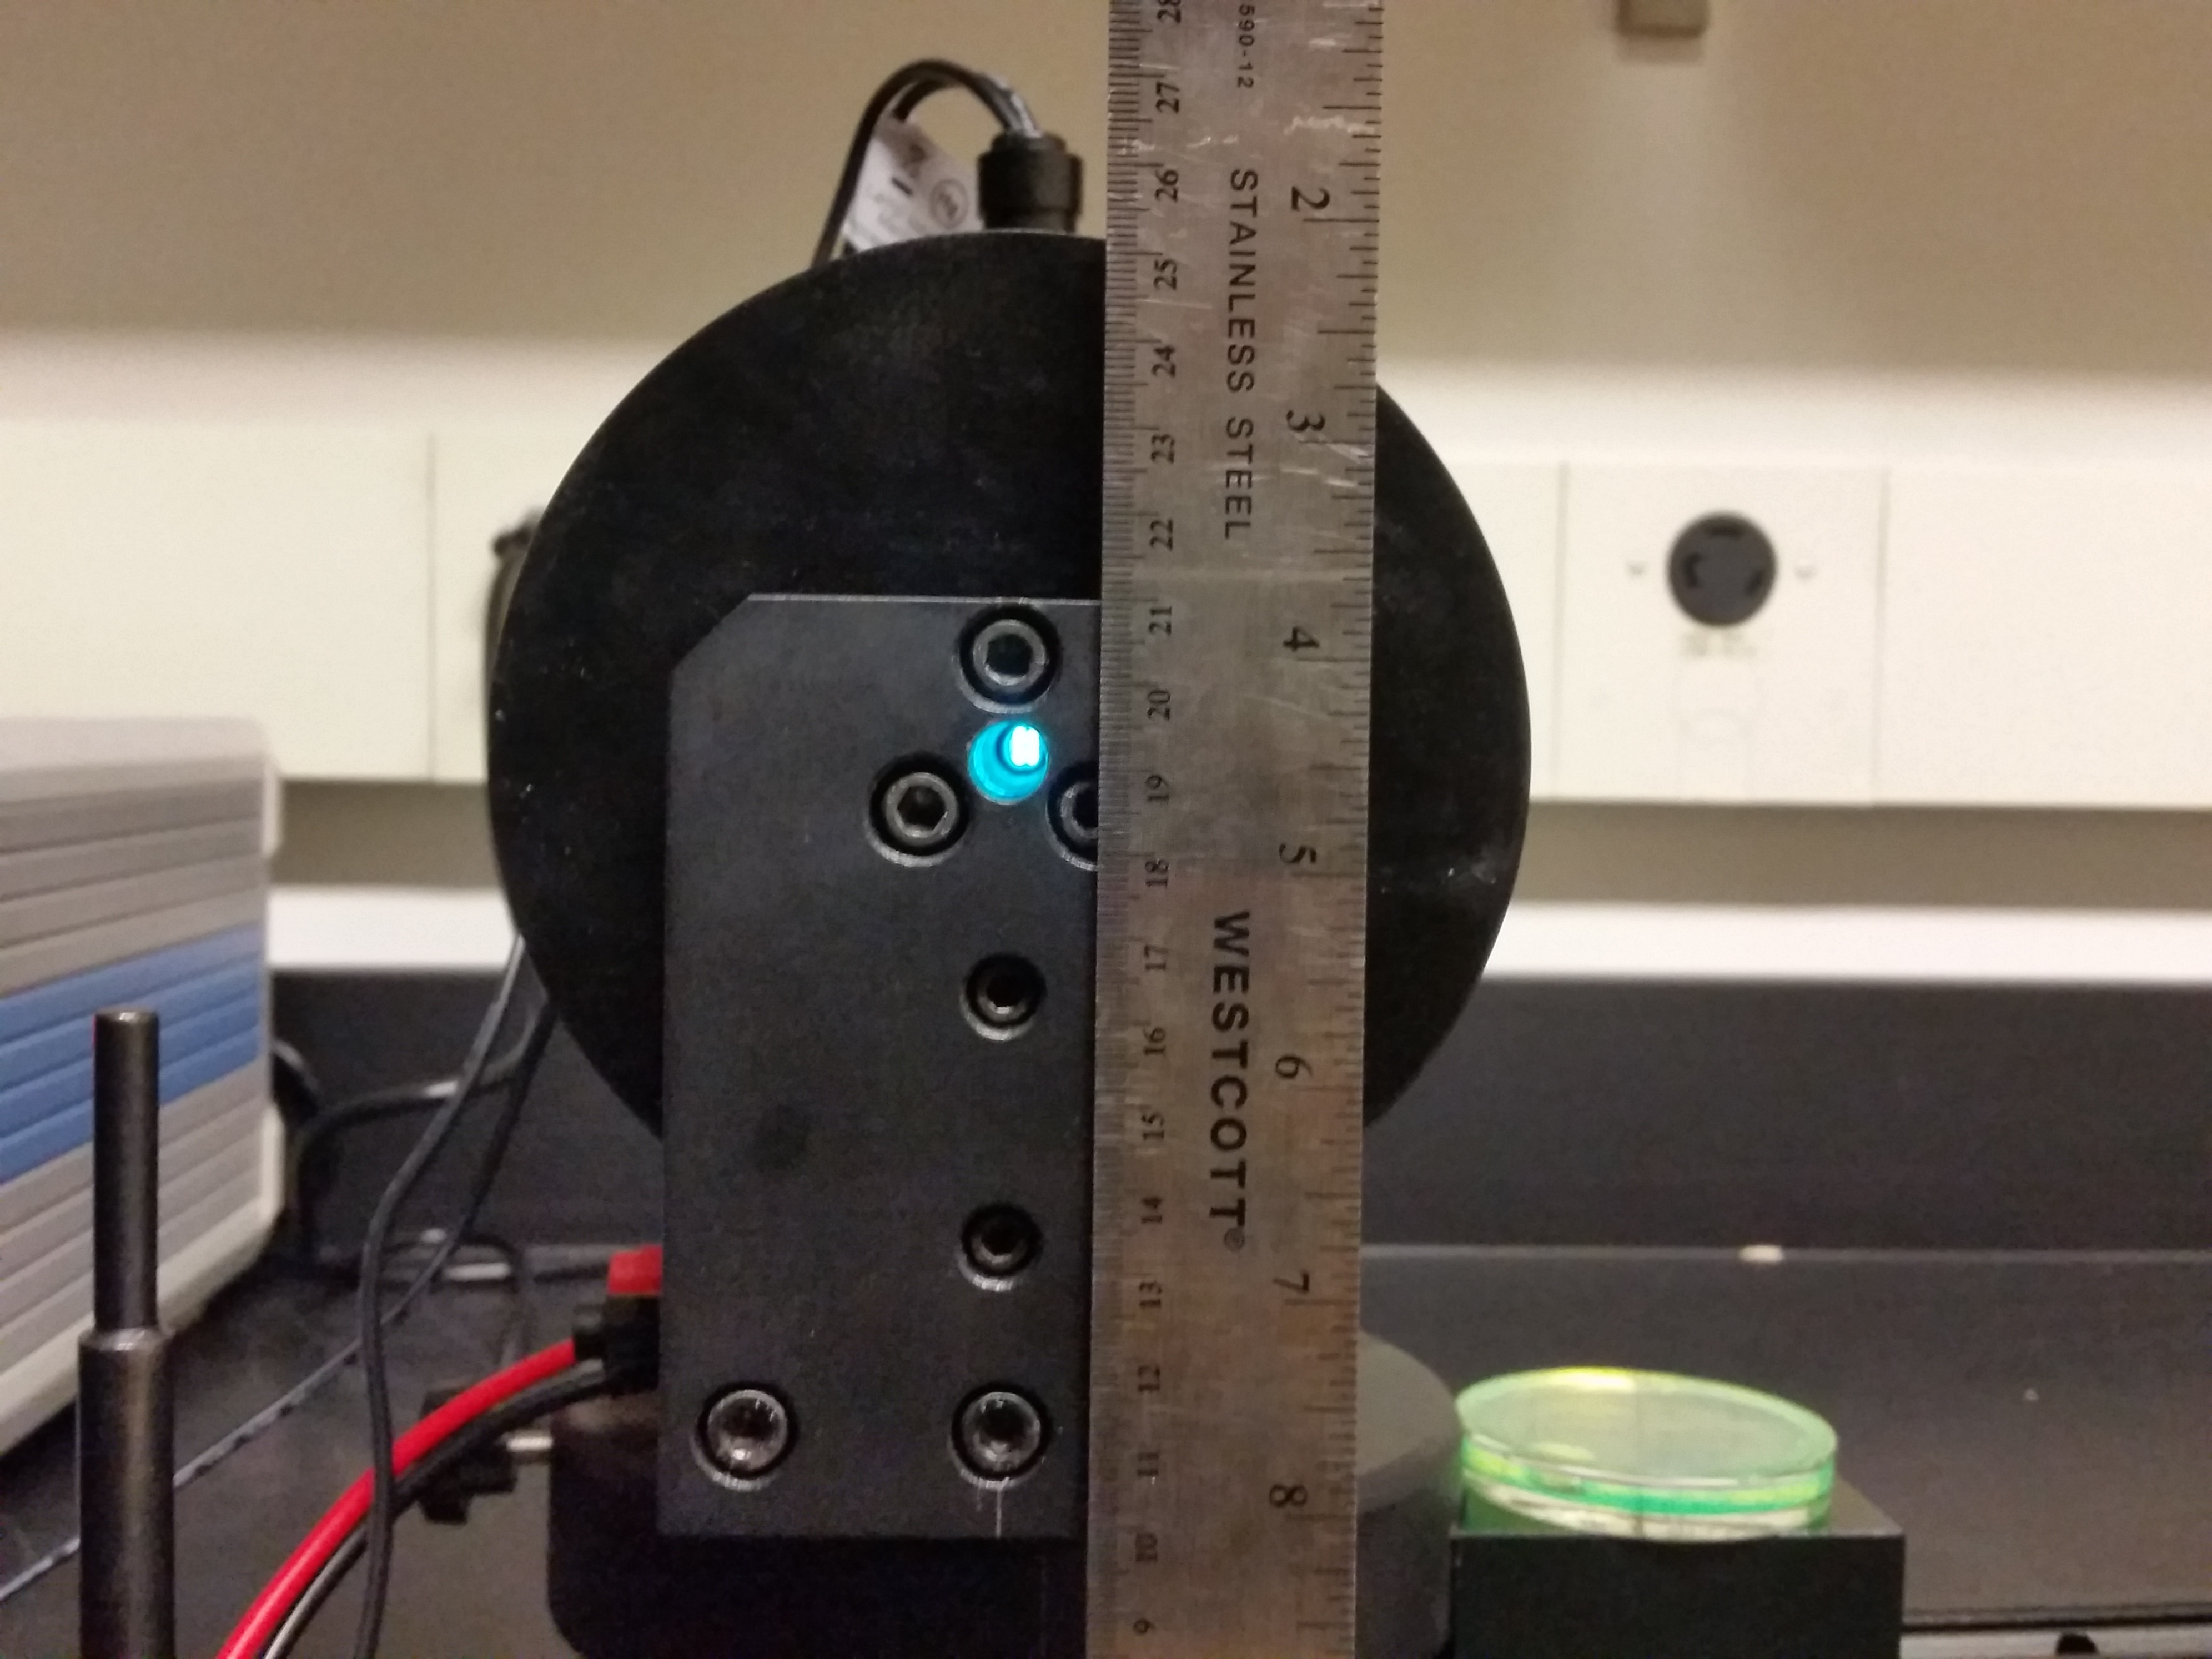
\includegraphics[width = 0.8\textwidth]{Images/AxialView.jpg}
			\caption{}
			\label{subfig:AxialView}
		\end{subfigure}%
		\caption{\textbf{Detail view of the solenoid with the mercury lamp source. Figure \ref{subfig:PerpView} shows the configuration with the magnetic field lines perpendicular to the light source. Figure \ref{subfig:AxialView} shows the axial field configuration looking down the sight-hole of the solenoid to the mercury lamp.}}
		\label{fig:SolenoidDetail}
	\end{figure*}
	
	
	
	To study the Zeeman effect, observations of a mercury lamp were made first with no magnetic field and $90\deg$ polarization, then with an approximately $1T$ magnetic field.
	Observations with a magnetic field included:
	\begin{itemize}
		\item $90\deg$ (field-perpendicular) polarization
		\item $0\deg$ (field-parallel) polarization 
		\item No polarization
		\item Axial B-field at polarization varying from $90\deg$ to $0\deg$
	\end{itemize}
	
	Figure \ref{fig:FieldConfig} shows the perpendicular and axial configurations of the magnetic field used for the observations.
	
	The observations and results of each of these field configurations will be presented and discussed in Section \ref{sec:DataAndResults}.
	
	 
	
	
	\begin{figure*}
		\centering
		\begin{subfigure}{0.55\textwidth}
			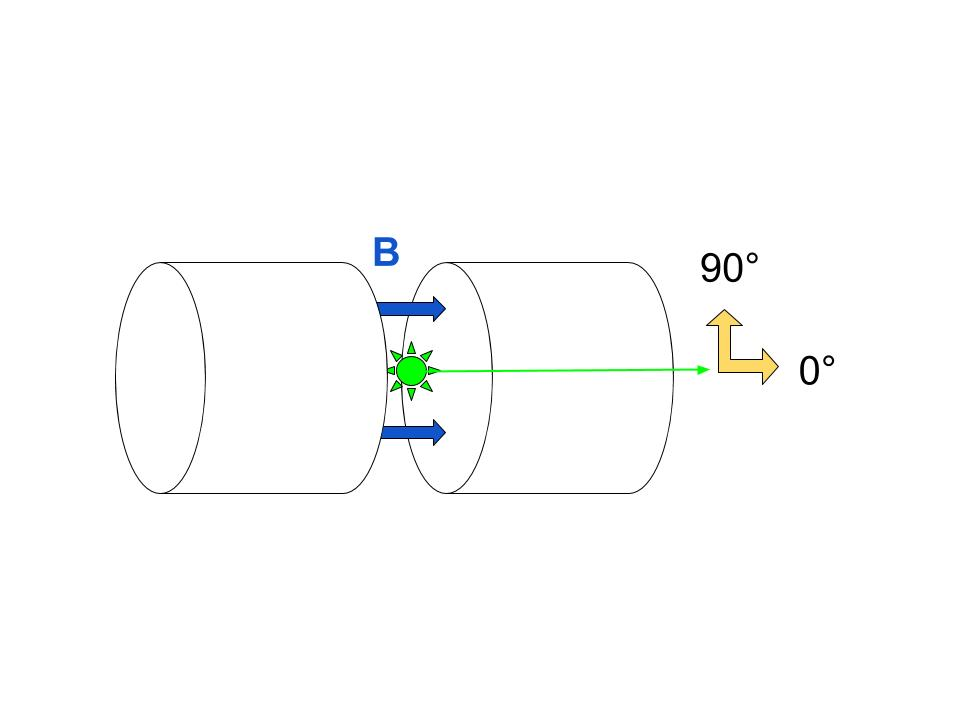
\includegraphics[width = 1.0\textwidth]{Images/FieldConfigA.jpg}
			\caption{\textbf{Perpendicular field configuration.}}
			\label{subfig:PerpFieldConfig}
		\end{subfigure}%
		\begin{subfigure}{0.55\textwidth}
			\centering
			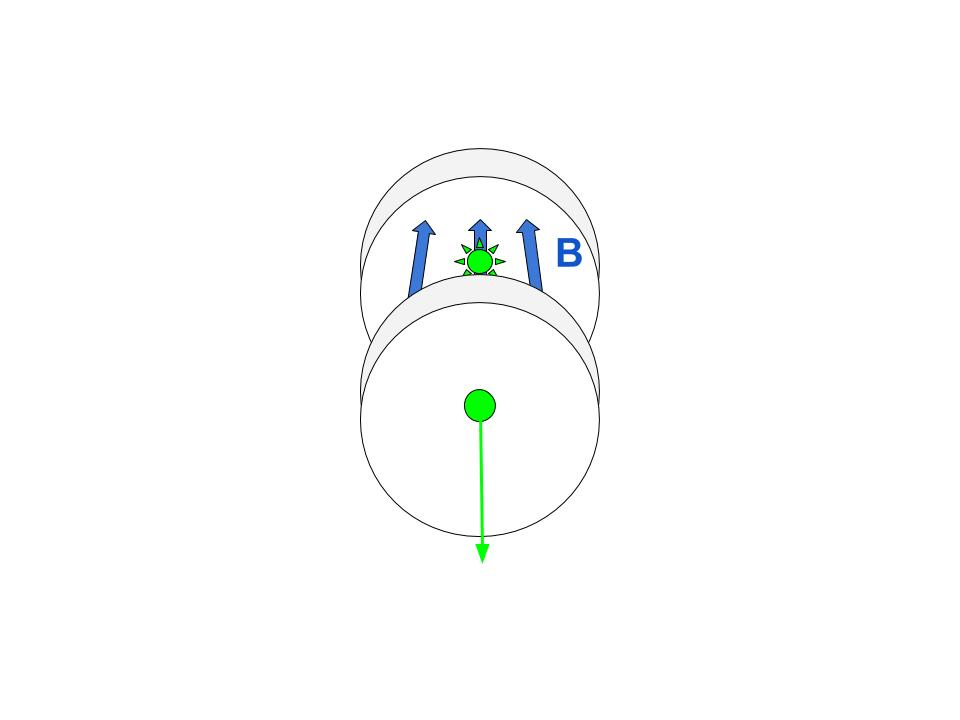
\includegraphics[width=1.0\textwidth]{Images/FieldConfigB.jpg}
			\caption{\textbf{Axial field configuration.}}
			\label{subfig:AxialFieldConfig}
		\end{subfigure}%
		\caption{\textbf{The two magnetic field configurations observed. In (\ref{subfig:PerpFieldConfig}), the magnetic field is oriented perpendicularly to the path of the observed light from the mercury lamp. $\mathbf{90\deg}$ polarization is defined to be perpendicular to the field lines, while $\mathbf{0\deg}$ polarization is parallel to the field lines. In configuration (\ref{subfig:AxialFieldConfig}), light from the lamp travels along the magnetic field lines down the center of one of the solenoids through a sight hole.}}
		\label{fig:FieldConfig}
	\end{figure*}
	
	\subsection{Method Description} \label{subsec:MethodDescription}
	
\section{Data and Results} \label{sec:DataAndResults}
	 
	 \begin{table}[h]
	 	\centering
	 	\begin{tabular}{l|l}
	 		k & Radius (m) \\ \hline
	 		4 & 0.7956 $\pm$ $0.1\times10^{-3}$    \\
	 		3 & 0.6911 $\pm$ $0.2\times10^{-3}$    \\
	 		2 & 0.5678 $\pm$ $0.1\times10^{-3}$    \\
	 		1 & 0.4096 $\pm$ $0.1\times10^{-3}$   
	 	\end{tabular}
	 	\caption{\textbf{Interference ring radii of the mercury 546.1 nm spectra with no magnetic field.}}
	 	\label{tab:B0Data}
	 	
	 \end{table}
	\subsection{Spectra Through a Perpendicular Magnetic Field}
		\subsubsection{Spectra with Field-Perpendicular Polarization}
			
			\begin{table*}[]
				\centering
				\begin{tabular}{l|lll}
					k = 1 & & & \\
					Measurements & $R+$ (m) & $R-$ (m)  & $\Delta$R (m) \\ \hline
					1         & 0.4282 & 0.3893  & 0.0389 \\
					2         & 0.4278 & 0.3896  & 0.0382 \\
					3         & 0.4275 & 0.3887  & 0.0388 \\
					Mean      & $0.4278\pm0.4\times10^{-3}$       & $0.3892\pm0.5\times10^{-3}$        & $0.039\pm0.4\times10^{-3}$ \\ \hline
					k = 2 & & & \\
					Measurements & $R+$ (m) & $R-$ (m)  & $\Delta$R (m) \\ \hline
					1           & 0.5819 & 0.5539 & 0.0280 \\
					2           & 0.5815 & 0.5536 & 0.0279 \\
					3           & 0.5818 & 0.5536 & 0.0282 \\
					Mean        & $0.5817\pm0.2\times10^{-3}$ & $0.5537\pm0.2\times10^{-3}$ & $0.0280\pm0.2\times10^{-3}$ \\ \hline
					k = 3 & & & \\
					Measurements & $R+$ (m) & $R-$ (m)  & $\Delta$R (m) \\ \hline
					1    & 0.7035 & 0.679  & 0.0245 \\
					2    & 0.7033 & 0.6798 & 0.0235 \\
					3    & 0.7025 & 0.6805 & 0.0220 \\
					Mean & $0.7031\pm0.5\times10^{-3}$ & $0.6798\pm0.8\times10^{-3}$ & $0.0233\pm0.001$ \\ \hline
					k = 4 & & & \\
					Measurements & $R+$ (m) & $R-$ (m)  & $\Delta$R (m) \\ \hline
					1    & 0.8058 & 0.7861 & 0.02  \\
					2    & 0.8057 & 0.7865 & 0.02  \\
					3    & 0.8059 & 0.7857 & 0.02  \\
					Mean & $0.8058\pm0.1\times10^{-3}$ & $0.7861\pm0.4\times10^{-3}$ & $0.020\pm0.001$
				\end{tabular}
				
				
				\caption{\textbf{Radius measurements of the hyperfine structure of the k=1 through k=4 interference rings with a 1T magnetic field and $\mathbf{90\degree}$ polarization.}}
				\label{my-label}
			\end{table*}
			
		\subsubsection{Spectra with Field-Parallel Polarization}
	
	\subsection{Spectra Along an Axial Magnetic Field}
	
	\subsection{Measurement of the Bohr Magneton} \label{subsec:BohrMagneton}
		With the precise measurement of spectral line splitting in the presence of the perpendicular magnetic field, it was possible to measure the value of the Bohr magneton.
		
		\begin{table}[]
			\centering
			\begin{tabular}{l|l}
				$\mathbf{k}$    & $\mathbf{\mu_B \ (J/T)}$ \\ \hline
				\textbf{1}    & $9.16\times10^{-24}$   \\
				\textbf{2}    & $9.24\times10^{-24}$   \\
				\textbf{3}    & $9.36\times10^{-24}$   \\
				\textbf{4}    & $9.10\times10^{-24}$   \\ \hline
				\textbf{Mean} & $9.22\times10^{-24}\pm0.6\times10^{-24}$  
			\end{tabular}
			\caption{\textbf{Calculated values of the Bohr magneton $\mathbf{\mu_B}$ for each interference ring, and the mean calculated value for all interference rings.}}
			\label{tab:BohrCalcs}
		\end{table}
	

\section{Conclusion} \label{sec:Conclusion}

\end{document}
